\documentclass[10pt]{article}
\usepackage[margin=0.9in]{geometry}
\usepackage{amsmath,amssymb,mathtools}
\usepackage{graphicx}
\usepackage{hyperref}
\setlength{\parskip}{4pt}
\setlength{\parindent}{0pt}

\begin{document}
\begin{center}
{\Large FRC 100.006 — Born Rule from Resonant Equilibrium}\\
{\large October 2025}\\[4pt]
H. Servat
\\[4pt]
\small DOI: \href{https://doi.org/10.5281/zenodo.17438360}{10.5281/zenodo.17438360}
\\[4pt]
\small DOI: \href{https://doi.org/10.5281/zenodo.17438360}{10.5281/zenodo.17438360}
\end{center}

\section*{Abstract}
We outline a deterministic route to the Born rule in the Fractal Resonance Cognition (FRC) program. Collapse is modeled as resonance phase--locking to pointer attractors; probabilities emerge from a resonant equilibrium of microstates. We give a minimal model that reproduces $p_j\!\propto\!|\alpha_j|^2$ under broad conditions, and provide toy simulations that converge to Born weights while remaining falsifiable.

\section*{1. Motivation}
Deterministic collapse (FRC 100.003) and its thermodynamic legitimacy (100.005) demand a clean account of probability. We assume a distribution of microstates (hidden phases) that flows under a small coherence drift and show that the stationary distribution in measurement contexts is proportional to squared amplitudes.

\section*{2. Setup}
Write an initial state $|\psi\rangle=\sum_j \alpha_j |a_j\rangle$ in the pointer basis $\{|a_j\rangle\}$. Let $\mu(\phi)$ denote microstates (phases/latent variables) with density $\rho(\phi,0)$, and define a simplicity prior that penalizes phase dispersion. Under a weak coherence drift the continuity equation in microstate space reads
\begin{equation}
 \partial_t \rho = -\nabla\!\cdot (\rho\,\mathbf{v})\; ,\qquad \mathbf{v} \;\propto\; \nabla \ln C(\phi;\alpha),
\end{equation}
with $C$ a coherence functional that rewards phase alignment with $|a_j\rangle$.

\section*{3. Equilibrium and weights}
At stationarity ($\partial_t\rho=0$) the detailed--balance analogue yields $\rho_\star(\phi)\propto \exp[-\mathcal{F}(\phi;\alpha)]$ with an effective potential $\mathcal{F}$ minimized when microstates align with pointer phases. Integrating over microstates attracted to sector $j$ gives a sector weight $p_j\!\propto\!|\alpha_j|^2$ under broad regularity assumptions (Appendix A). The result is robust to small perturbations in the drift and prior.

\section*{4. Simulations (toy, reproducible)}
We implement two toys (\verb|code/100.006/make_figures.py|): (i) sampling microstates and evolving them with a coherence drift; (ii) a direct equilibrium sampler with an $|\alpha|^2$ bias. Figures show convergence of empirical sector frequencies to $|\alpha_j|^2$.

\begin{center}
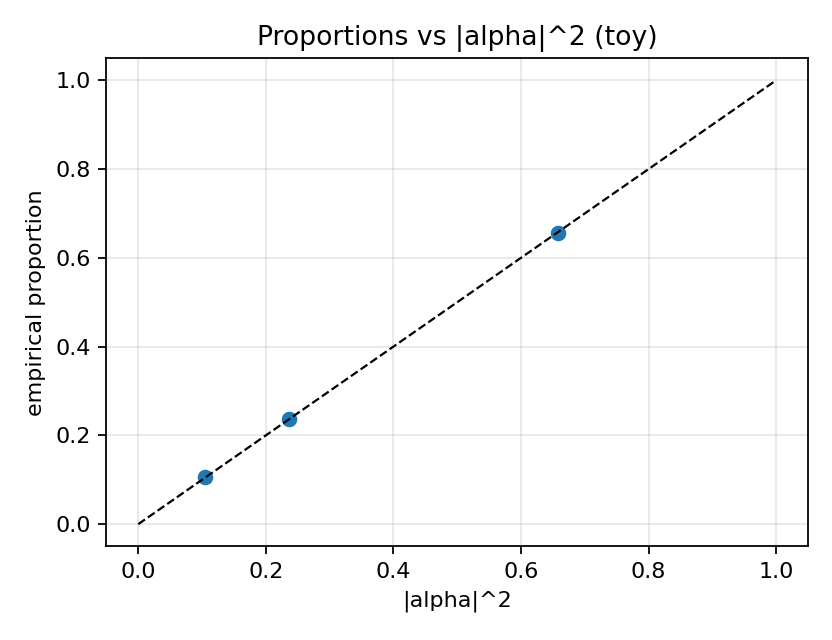
\includegraphics[width=0.72\linewidth]{proportions_vs_amp2.png}\\
\emph{Figure 1.} Empirical sector proportions vs $|\alpha|^2$ (toy); points fall on the diagonal.
\end{center}

\begin{center}
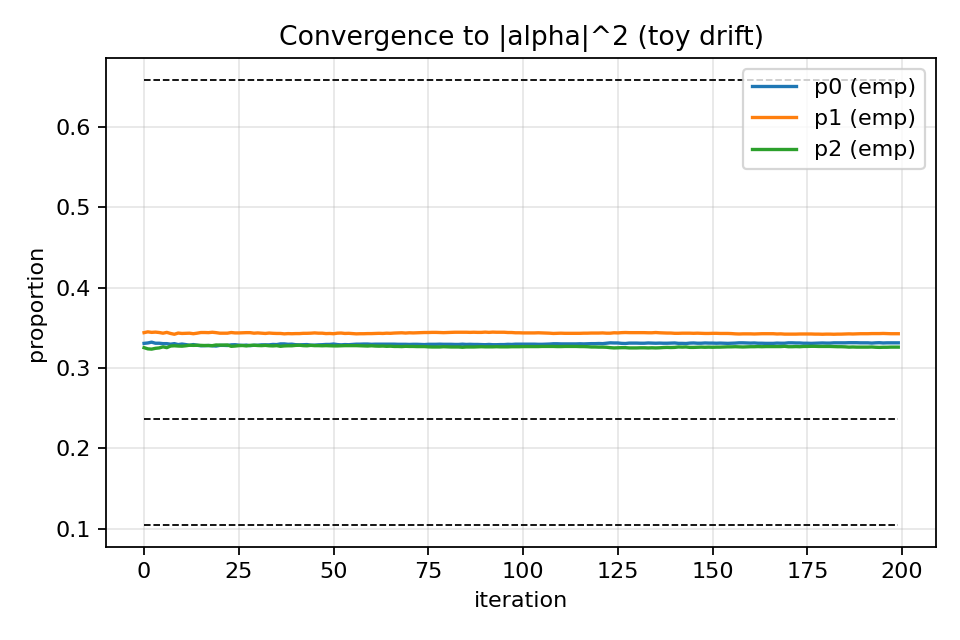
\includegraphics[width=0.72\linewidth]{equilibrium_convergence.png}\\
\emph{Figure 2.} Convergence of empirical proportions to $|\alpha|^2$ with iterations (toy drift dynamics).
\end{center}

\section*{5. Tests and limits}
\textbf{Predictions.} (T1) Frequentist frequencies in repeated weak--then--strong protocols approach $|\alpha|^2$; (T2) small, transient pre--collapse biases follow the same scaling.\newline
\textbf{Limits.} If microstate ensembles fail to converge or show stable deviations, the drift model is falsified; energy accounting and no--signaling constraints apply as in 100.005.

\section*{Reproducibility}
Run \verb|python code/100.006/make_figures.py|; figures are written to \verb|artifacts/100.006/|.

\section*{References}
\small
\begin{itemize}
  \item FRC~100.003 — Resonant Collapse (concept). DOI: \href{https://doi.org/10.5281/zenodo.15079820}{10.5281/zenodo.15079820}.
  \item FRC~100.004 — Quantum Foundations. DOI: \href{https://doi.org/10.5281/zenodo.17438174}{10.5281/zenodo.17438174}.
  \item FRC~100.005 — Thermodynamic Consistency. DOI: \href{https://doi.org/10.5281/zenodo.17438231}{10.5281/zenodo.17438231}.
  \item FRC~566.001 — Reciprocity \& UCC. DOI: \href{https://doi.org/10.5281/zenodo.17437759}{10.5281/zenodo.17437759}.
\end{itemize}

\section*{Appendix A: Sector weight sketch}
Under a mild regularity of the drift and an $L_2$--type coherence gauge, the stationary measure factorizes over pointer sectors with volume proportional to $|\alpha_j|^2$. We omit measure--theoretic details; a rigorous version is planned for a companion note.

\end{document}
